\documentclass[12pt,a4paper]{article}

\usepackage[margin=2.5cm]{geometry}
\usepackage{amsmath}
\usepackage{listings}
\usepackage{xcolor}
\usepackage{titlesec}
\usepackage{parskip}
\usepackage{hyperref}
\usepackage{booktabs}
\usepackage{array}
\usepackage{enumitem}
\usepackage{fancyhdr}
\usepackage{mdframed}
\usepackage{tikz}
\usetikzlibrary{shapes.geometric, arrows.meta, positioning, fit, backgrounds, calc}
\setlength{\headheight}{13.6pt}
\addtolength{\topmargin}{-1.6pt}

% --- colours ---
\definecolor{codebg}{rgb}{0.96,0.96,0.96}
\definecolor{codeframe}{rgb}{0.75,0.75,0.75}
\definecolor{keywordcolor}{rgb}{0.0,0.35,0.65}
\definecolor{commentcolor}{rgb}{0.4,0.4,0.4}
\definecolor{stringcolor}{rgb}{0.13,0.54,0.13}
\definecolor{noteblue}{rgb}{0.88,0.93,0.98}
\definecolor{noteframe}{rgb}{0.3,0.5,0.8}
\definecolor{warnbg}{rgb}{1.0,0.95,0.88}
\definecolor{warnframe}{rgb}{0.85,0.55,0.1}

% --- listings style ---
\lstdefinestyle{pycode}{
  language=Python,
  backgroundcolor=\color{codebg},
  frame=single,
  rulecolor=\color{codeframe},
  basicstyle=\ttfamily\small,
  keywordstyle=\color{keywordcolor}\bfseries,
  commentstyle=\color{commentcolor}\itshape,
  stringstyle=\color{stringcolor},
  breaklines=true,
  showstringspaces=false,
  tabsize=4,
  numbers=left,
  numberstyle=\tiny\color{commentcolor},
  numbersep=6pt,
}

\lstdefinestyle{jsoncode}{
  backgroundcolor=\color{codebg},
  frame=single,
  rulecolor=\color{codeframe},
  basicstyle=\ttfamily\small,
  breaklines=true,
  showstringspaces=false,
}

\lstdefinestyle{plaincode}{
  backgroundcolor=\color{codebg},
  frame=single,
  rulecolor=\color{codeframe},
  basicstyle=\ttfamily\small,
  breaklines=true,
}

% --- note boxes ---
\newmdenv[
  backgroundcolor=noteblue,
  linecolor=noteframe,
  linewidth=1.5pt,
  innerleftmargin=10pt,
  innerrightmargin=10pt,
  innertopmargin=8pt,
  innerbottommargin=8pt,
  skipabove=10pt,
  skipbelow=10pt,
]{notebox}

\newmdenv[
  backgroundcolor=warnbg,
  linecolor=warnframe,
  linewidth=1.5pt,
  innerleftmargin=10pt,
  innerrightmargin=10pt,
  innertopmargin=8pt,
  innerbottommargin=8pt,
  skipabove=10pt,
  skipbelow=10pt,
]{warnbox}

% --- headers ---
\pagestyle{fancy}
\fancyhf{}
\rhead{\small Graph-Based Agent Orchestration — Study Notes}
\lhead{\small TSAI EAG V3 · Week 9}
\rfoot{\thepage}

\titleformat{\section}{\large\bfseries}{}{0em}{}[\titlerule]
\titleformat{\subsection}{\normalsize\bfseries}{}{0em}{}

\hypersetup{
  colorlinks=true,
  linkcolor=keywordcolor,
  urlcolor=keywordcolor,
}

% ─────────────────────────────────────────────────────────────────────────────

\begin{document}

\begin{titlepage}
  \centering
  \vspace*{3cm}
  {\Huge\bfseries Graph-Based Agent Orchestration\\[0.5em]}
  {\Large Study Notes for Interview Preparation\\[2em]}
  \rule{10cm}{0.5pt}\\[1.5em]
  {\large TSAI EAG V3 — Week 9, Assignment 9}\\[0.5em]
  {\large Session 8 / Session 9 Agent System}\\[2em]
  \rule{10cm}{0.5pt}\\[1.5em]
  {\normalsize Topics covered: DAG execution, Planner role, skill isolation,\\
  node failure, recovery replanning, orchestrator definition,\\
  LLM context management}\\[3cm]
  {\small Prepared for interview study}
\end{titlepage}

\tableofcontents
\newpage

% ─────────────────────────────────────────────────────────────────────────────
\section{System Overview}
% ─────────────────────────────────────────────────────────────────────────────

The assignment contains two major components that work together:

\begin{center}
\begin{tabular}{>{\bfseries}p{4.5cm} p{9cm}}
\toprule
Component & Purpose \\
\midrule
\texttt{llm\_gatewayV9/} & A FastAPI-based multi-provider LLM routing gateway.
  Handles provider failover, rate limiting, streaming, tool calls, embeddings,
  vision, and structured output. \\[0.5em]
\texttt{S9SharedCode/code/} & A graph-based multi-skill agentic orchestrator.
  Decomposes user queries into a DAG of skills, executes them with dependency
  ordering, handles failure recovery, and maintains persistent session state. \\
\bottomrule
\end{tabular}
\end{center}

The orchestrator calls the gateway for every LLM interaction. From the
orchestrator's perspective, the gateway is a black box: send a prompt, get text
back.

% ─────────────────────────────────────────────────────────────────────────────
\section{What is an Orchestrator?}
% ─────────────────────────────────────────────────────────────────────────────

\begin{notebox}
\textbf{Definition.} An \textbf{orchestrator} is the component that manages the
execution of a multi-step workflow. It decides \emph{what runs, when, and with
what inputs} — without doing the actual work itself.
\end{notebox}

In this codebase the \texttt{Executor} class in \texttt{flow.py} is the
orchestrator. Its job is purely mechanical:

\begin{enumerate}[noitemsep]
  \item Look at the graph $\rightarrow$ find which nodes are \emph{ready}
  \item Fire those nodes (hand each one to its LLM)
  \item Collect results $\rightarrow$ update node statuses
  \item Extend the graph if new nodes were emitted
  \item Repeat until nothing is left to run
\end{enumerate}

The orchestrator never reasons about the query. It does not know what
``researcher'' or ``distiller'' means semantically. It just moves work through
the graph.

\subsection{Kitchen Analogy}

\begin{center}
\begin{tabular}{>{\bfseries}p{4cm} p{9cm}}
\toprule
Role & Analogy \\
\midrule
Orchestrator & Head chef calling out orders: \emph{``table 3's starter is
  ready, fire the main''} \\
Skills (LLMs) & Individual cooks — each one only knows their station \\
Graph & The order ticket — what depends on what \\
\midrule
\multicolumn{2}{l}{\small The head chef never cooks. The cooks never read
other stations' tickets.} \\
\bottomrule
\end{tabular}
\end{center}

More formally: an orchestrator sits \textbf{above} the workers and
\textbf{below} the user. It translates a high-level goal (the DAG) into a
sequence of concrete, scoped calls — handling parallelism, failure, and
ordering — so that no individual worker needs to know about the bigger picture.

% ─────────────────────────────────────────────────────────────────────────────
\section{Key Concepts}
% ─────────────────────────────────────────────────────────────────────────────

\subsection{The Graph}

The agent's execution plan is a \textbf{NetworkX directed acyclic graph (DiGraph)}.
Each node represents one skill invocation. Edges encode data dependencies:
an edge $A \rightarrow B$ means ``$B$ must wait for $A$ to complete before it
can run, and $B$ will receive $A$'s output as input.''

\begin{lstlisting}[style=pycode, caption={Graph node structure (flow.py)}]
def add_node(self, skill: str, inputs: list[str], metadata: dict | None = None) -> str:
    self._counter += 1
    nid = f"n:{self._counter}"
    self.g.add_node(nid, skill=skill, inputs=list(inputs),
                    metadata=dict(metadata or {}), status="pending")
    for inp in inputs:
        if inp.startswith("n:") and inp in self.g.nodes:
            self.g.add_edge(inp, nid)   # edge = data dependency
    return nid
\end{lstlisting}

Each node carries:
\begin{itemize}[noitemsep]
  \item \textbf{skill} — which skill type to run (\texttt{researcher}, \texttt{distiller}, etc.)
  \item \textbf{inputs} — list of upstream node IDs or special literals
  \item \textbf{status} — \texttt{pending / running / complete / failed / skipped}
  \item \textbf{metadata} — opaque dict (labels, sub-questions, failure reports)
  \item \textbf{result} — populated after execution (\texttt{AgentResult})
\end{itemize}

\subsection{Ready Nodes}

A node is \textbf{ready} when all its predecessors are either
\texttt{complete} or \texttt{skipped}:

\begin{lstlisting}[style=pycode, caption={ready\_nodes() — flow.py}]
def ready_nodes(self) -> list[str]:
    out = []
    for nid, d in self.g.nodes(data=True):
        if d["status"] != "pending":
            continue
        preds = list(self.g.predecessors(nid))
        if all(self.g.nodes[p]["status"] in ("complete", "skipped") for p in preds):
            out.append(nid)
    return out
\end{lstlisting}

\begin{warnbox}
\textbf{Important:} A \texttt{failed} predecessor does NOT satisfy the
``complete or skipped'' check. A node whose predecessor is \texttt{failed}
will \emph{never} become ready and will be left behind in the graph when
the loop exits.
\end{warnbox}

\subsection{Skills Catalogue}

\begin{center}
\begin{tabular}{>{\ttfamily}p{3.5cm} p{4.5cm} p{5cm}}
\toprule
\normalfont\textbf{Skill} & \textbf{Purpose} & \textbf{Special flags} \\
\midrule
planner      & Decomposes query into DAG & Main planning entry point \\
researcher   & Web search + fetch        & \texttt{tools\_allowed: [web\_search, fetch\_url]} \\
retriever    & FAISS knowledge search    & \texttt{tools\_allowed: [search\_knowledge]} \\
distiller    & Structured extraction     & \texttt{critic: true} \\
summariser   & Condense long content     & --- \\
critic       & Pass/fail evaluator       & Auto-inserted by orchestrator \\
formatter    & Final answer renderer     & Terminal node \\
coder        & Emit Python code          & \texttt{internal\_successors: [sandbox\_executor]} \\
sandbox\_executor & Run code in sandbox  & Bypasses LLM entirely \\
browser      & JS-rendered page fetching & Bypasses LLM gateway \\
\bottomrule
\end{tabular}
\end{center}

% ─────────────────────────────────────────────────────────────────────────────
\section{The Planner's Role}
% ─────────────────────────────────────────────────────────────────────────────

\begin{notebox}
\textbf{Key insight.} The Planner emits the \textbf{entire DAG upfront} in a
single LLM call — not just the next step. Every node, every branch, and every
dependency edge is defined before any worker node runs.
\end{notebox}

\subsection{Common Misconception}

\begin{center}
\begin{tabular}{p{6cm} p{6cm}}
\toprule
\textbf{Wrong mental model} & \textbf{Actual behaviour} \\
\midrule
Planner $\rightarrow$ Researcher decides next $\rightarrow$ Distiller decides next $\rightarrow$ Formatter

\smallskip
Each skill picks its own successor at runtime (a chain). &

Planner emits all nodes at once. Workers run in dependency order. No worker decides what runs after it.

\smallskip
The DAG topology is fixed by the Planner. Workers are just data processors. \\
\bottomrule
\end{tabular}
\end{center}

\subsection{What the Planner Returns}

\begin{lstlisting}[style=jsoncode, caption={Typical Planner JSON output}]
{
  "successors": [
    {"skill": "researcher", "inputs": ["USER_QUERY"],
     "metadata": {"label": "tokyo", "question": "Population of Tokyo?"}},
    {"skill": "researcher", "inputs": ["USER_QUERY"],
     "metadata": {"label": "paris", "question": "Population of Paris?"}},
    {"skill": "distiller",  "inputs": ["n:tokyo", "n:paris"],
     "metadata": {"label": "distiller"}},
    {"skill": "formatter",  "inputs": ["n:distiller"]}
  ]
}
\end{lstlisting}

All four nodes are added to the graph immediately. The Planner's job is done.

\subsection{Three Ways the Graph Can Grow}

These are processed in \texttt{Graph.extend\_from()} after any node completes:

\begin{enumerate}
  \item \textbf{Dynamic successors} (\texttt{result.successors}) — what the
    skill's LLM output explicitly requested. This is meaningful mainly for the
    Planner. Workers rarely emit successors.

  \item \textbf{Static internal successors} (\texttt{internal\_successors} in
    \texttt{agent\_config.yaml}) — unconditional. Example: \texttt{coder} always
    appends \texttt{sandbox\_executor}.

  \item \textbf{Critic auto-insertion} — when a skill with \texttt{critic: true}
    (e.g.\ \texttt{distiller}) completes, the orchestrator automatically inserts
    a \texttt{critic} node between it and every outgoing child. No skill
    requested this — the orchestrator enforces it.
\end{enumerate}

% ─────────────────────────────────────────────────────────────────────────────
\section{Normal DAG Execution — Full Example}
% ─────────────────────────────────────────────────────────────────────────────

\textbf{Query:} \textit{``Compare the population of Tokyo and Paris''}

\subsection{Initial State}

\begin{lstlisting}[style=pycode]
graph.add_node("planner", inputs=["USER_QUERY"])
# Graph: n:1  planner  status=pending
\end{lstlisting}

\subsection{Iteration 1 — Planner runs}

\texttt{ready\_nodes()} returns \texttt{[n:1]} — no predecessors.

The Planner LLM receives only \texttt{USER\_QUERY}. It emits four successor
nodes. \texttt{extend\_from()} resolves labels and builds edges:

\begin{lstlisting}[style=plaincode]
n:1  planner    complete
n:2  researcher pending   inputs=[USER_QUERY]         (Tokyo)
n:3  researcher pending   inputs=[USER_QUERY]         (Paris)
n:4  distiller  pending   inputs=[n:2, n:3]
n:5  formatter  pending   inputs=[n:4]

Edges: n:1->n:2, n:1->n:3, n:2->n:4, n:3->n:4, n:4->n:5
\end{lstlisting}

\begin{center}
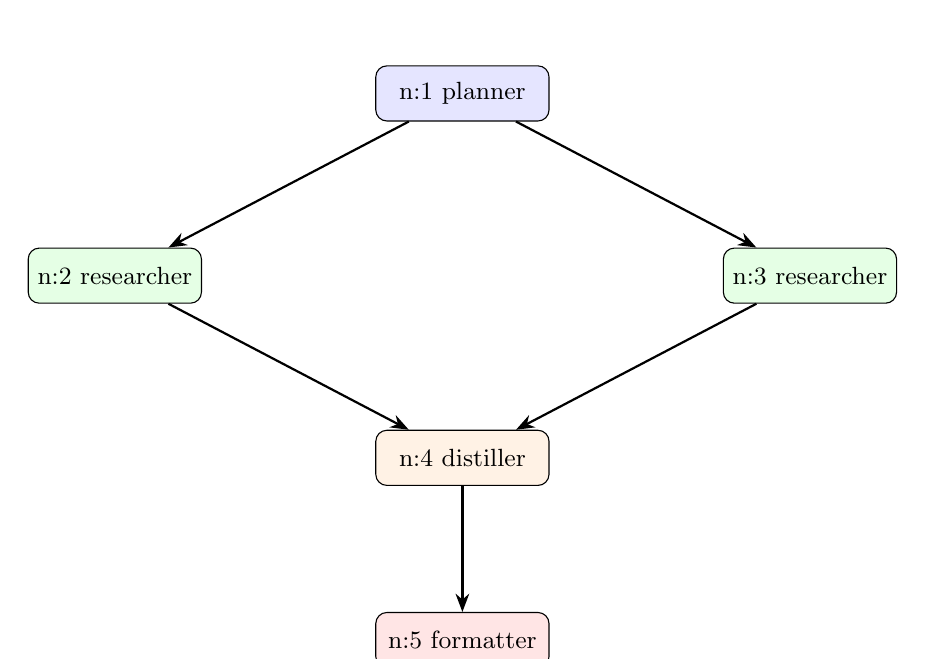
\begin{tikzpicture}[
  node distance=1.6cm and 2.2cm,
  every node/.style={draw, rounded corners, minimum width=2.2cm, minimum height=0.7cm,
    font=\small, fill=white},
  arrow/.style={-Stealth, thick},
]
  \node (p) [fill=blue!10] {n:1 planner};
  \node (r1) [below left=of p, fill=green!10] {n:2 researcher};
  \node (r2) [below right=of p, fill=green!10] {n:3 researcher};
  \node (d)  [below right=of r1, fill=orange!10] {n:4 distiller};
  \node (f)  [below=of d, fill=red!10] {n:5 formatter};

  \draw[arrow] (p)  -- (r1);
  \draw[arrow] (p)  -- (r2);
  \draw[arrow] (r1) -- (d);
  \draw[arrow] (r2) -- (d);
  \draw[arrow] (d)  -- (f);
\end{tikzpicture}
\end{center}

\subsection{Iteration 2 — Both Researchers Run in Parallel}

\texttt{ready\_nodes()} returns \texttt{[n:2, n:3]} — both have only \texttt{n:1}
as predecessor, which is \texttt{complete}.

\begin{lstlisting}[style=pycode, caption={Parallel execution — flow.py:251}]
outcomes = await asyncio.gather(*[
    self._run_one("n:2", ...),   # Tokyo researcher
    self._run_one("n:3", ...)    # Paris researcher
])
\end{lstlisting}

They run simultaneously. Neither emits successors. Graph after:

\begin{lstlisting}[style=plaincode]
n:2  researcher  complete   output={"findings": "Tokyo population is 13.96M..."}
n:3  researcher  complete   output={"findings": "Paris population is 2.16M..."}
n:4  distiller   pending    (still waiting)
n:5  formatter   pending    (still waiting)
\end{lstlisting}

\subsection{Iteration 3 — Distiller Runs, Critic Auto-inserted}

\texttt{ready\_nodes()} returns \texttt{[n:4]} — predecessors \texttt{n:2} and
\texttt{n:3} are both \texttt{complete}.

The distiller's rendered prompt contains the outputs of \textbf{both}
researchers in its \texttt{INPUTS} block. It produces structured data.

After \texttt{extend\_from()}, the critic auto-insertion fires because
\texttt{distiller} has \texttt{critic: true}:

\begin{lstlisting}[style=pycode, caption={Critic auto-insertion — flow.py:161--179}]
# remove edge n:4 -> n:5
# insert n:6 (critic) with inputs=[USER_QUERY, n:4]
# add edges: n:4->n:6, n:6->n:5
\end{lstlisting}

Graph after:

\begin{lstlisting}[style=plaincode]
n:4  distiller  complete   output={"tokyo_pop": "13.96M", "paris_pop": "2.16M"}
n:6  critic     pending    inputs=[USER_QUERY, n:4]   <- auto-inserted
n:5  formatter  pending    inputs=[n:4]               <- now gated behind n:6
\end{lstlisting}

\subsection{Iteration 4 — Critic Evaluates}

\texttt{ready\_nodes()} returns \texttt{[n:6]}.

Critic receives \texttt{USER\_QUERY} and \texttt{n:4}'s output. It emits
\texttt{\{"verdict": "pass"\}}. \texttt{handle\_critic\_verdict} sees
\texttt{"pass"} $\rightarrow$ returns \texttt{False} $\rightarrow$ normal flow
continues. \texttt{n:5} becomes ready.

\subsection{Iteration 5 — Formatter Produces Final Answer}

\texttt{ready\_nodes()} returns \texttt{[n:5]}.

Formatter receives only \texttt{n:4}'s clean structured output. It produces:
\begin{lstlisting}[style=jsoncode]
{"final_answer": "Tokyo (13.96M) is approximately 6x larger than Paris (2.16M)."}
\end{lstlisting}

The orchestrator captures this:
\begin{lstlisting}[style=pycode]
if graph.g.nodes[nid]["skill"] == "formatter":
    fa = result.output.get("final_answer")
    if isinstance(fa, str) and fa.strip():
        formatter_answer = fa
\end{lstlisting}

\subsection{Iteration 6 — Loop Exits}

\begin{lstlisting}[style=pycode]
while True:
    ready = graph.ready_nodes()
    if not ready and not graph.has_running():
        break   # exits here
\end{lstlisting}

\subsection{Execution Summary}

\begin{center}
\begin{tabular}{>{\bfseries}p{1.5cm} p{4cm} p{7cm}}
\toprule
Iteration & Nodes running & Key event \\
\midrule
1 & n:1 planner        & Full DAG built from USER\_QUERY \\
2 & n:2, n:3 parallel  & Both researchers fire simultaneously \\
3 & n:4 distiller      & Critic auto-inserted after completion \\
4 & n:6 critic         & Evaluates distiller; verdict = pass \\
5 & n:5 formatter      & Final answer produced \\
6 & (none)             & Loop exits \\
\bottomrule
\end{tabular}
\end{center}

% ─────────────────────────────────────────────────────────────────────────────
\section{LLM Context Isolation}
% ─────────────────────────────────────────────────────────────────────────────

\begin{notebox}
\textbf{Each LLM call only sees the outputs of its explicitly wired input
nodes — not the entire graph.}
\end{notebox}

The key line is in \texttt{skills.py}:

\begin{lstlisting}[style=pycode, caption={Context is scoped to node inputs only — skills.py:266}]
resolved = resolve_inputs(graph_nodes[node_id]["inputs"], graph_nodes, query)
#                                    ^^^^^^^^^^^^^^^^^^^^
#                         ONLY this node's input list, not all graph nodes
\end{lstlisting}

\texttt{graph\_nodes} (the full graph) is passed in, but only
\texttt{graph\_nodes[node\_id]["inputs"]} is resolved. Everything else is
ignored.

\subsection{What Each Node Actually Receives}

\begin{center}
\begin{tabular}{>{\ttfamily\small}p{2.8cm} >{\ttfamily\small}p{2.8cm} p{6.5cm}}
\toprule
\normalfont\textbf{Node} & \normalfont\textbf{Inputs wired} & \normalfont\textbf{Context in prompt} \\
\midrule
n:2 researcher & {[}USER\_QUERY{]} & Query text only \\
n:3 researcher & {[}USER\_QUERY{]} & Query text only \\
n:4 distiller  & {[}n:2, n:3{]}   & Outputs of n:2 and n:3 only. No USER\_QUERY, no planner output \\
n:5 formatter  & {[}n:4{]}        & Output of n:4 only. Does not see raw researcher findings \\
\bottomrule
\end{tabular}
\end{center}

\subsection{One Shared Element: Memory Hits}

FAISS memory hits are read \textbf{once} at session start and passed to
\emph{every} skill's prompt:

\begin{lstlisting}[style=pycode, caption={Memory read once, shared across all nodes — flow.py:221}]
memory_hits = memory_svc.read(query) or []
# ... threaded into every run_skill call
\end{lstlisting}

This is capped at 8 hits ($\approx$400 chars each) — a small fixed overhead,
not the whole graph.

\subsection{Why This Matters}

\begin{itemize}[noitemsep]
  \item Context stays small and predictable per node
  \item Parallel nodes (\texttt{n:2} and \texttt{n:3}) have completely
    independent contexts — no cross-contamination
  \item A 10-node graph does not mean any single LLM sees 10$\times$ the tokens
  \item Cheap small models can be used for leaf nodes; smarter models only for
    the Planner
  \item The DAG structure is the orchestrator's concern — LLMs only see their
    slice
\end{itemize}

% ─────────────────────────────────────────────────────────────────────────────
\section{Node Failure and Recovery}
% ─────────────────────────────────────────────────────────────────────────────

\subsection{Recovery Philosophy}

\begin{notebox}
The graph is \textbf{never} serialised and passed to the recovery Planner.
Instead, the orchestrator extracts two things and injects them as the recovery
Planner node's inputs:
\begin{enumerate}[noitemsep]
  \item A short \textbf{failure report string} — what broke and why
  \item The \textbf{node IDs of all already-completed nodes} — their actual
    output data
\end{enumerate}
\end{notebox}

\subsection{Failure Classification — recovery.py}

\begin{lstlisting}[style=pycode, caption={Failure classifier — recovery.py:29--43}]
def classify_failure(error_text: str) -> RecoveryReason:
    transient_markers = ("503", "502", "504", "timeout", "connection", ...)
    if any(m in e for m in transient_markers):
        return "transient"
    if "malformed" in e or "validationerror" in e:
        return "validation_error"
    return "upstream_failure"
\end{lstlisting}

\subsection{Recovery Decision Table}

\begin{center}
\begin{tabular}{p{4.5cm} >{\bfseries}p{2cm} p{6cm}}
\toprule
\textbf{Failure reason} & \textbf{Action} & \textbf{Why} \\
\midrule
transient (503/timeout)    & skip    & Gateway already retried; no point replanning \\
validation\_error           & skip    & Prompt bug; fix the prompt, not the run \\
upstream\_failure + planner & skip    & Re-planning a planner would cause an infinite loop \\
upstream\_failure + other   & \textcolor{keywordcolor}{replan} & Queue a recovery Planner node \\
\bottomrule
\end{tabular}
\end{center}

\subsection{Recovery Example — n:3 Fails}

\textbf{Same query:} \textit{``Compare the population of Tokyo and Paris''}
\textbf{Failure:} \texttt{n:3} (Paris researcher) fails with
\texttt{"upstream parse error in content"}.

\textbf{Step 1 — classify:}
\begin{lstlisting}[style=plaincode]
classify_failure("upstream parse error in content")
# none of the transient markers match -> "upstream_failure"
\end{lstlisting}

\textbf{Step 2 — collect completed nodes:}
\begin{lstlisting}[style=pycode, caption={Collecting prior completed nodes — flow.py:304--310}]
prior_complete = [
    n for n, d in graph.g.nodes(data=True)
    if d.get("status") == "complete"
    and d["skill"] not in ("planner", "critic")   # skip routing nodes
    and isinstance(d.get("result"), AgentResult)
]
# prior_complete = ["n:2"]   <- only Tokyo researcher finished
\end{lstlisting}

\textbf{Step 3 — add recovery Planner node:}
\begin{lstlisting}[style=pycode, caption={Adding recovery Planner — flow.py:311--321}]
rec_nid = graph.add_node(
    "planner",
    inputs=["USER_QUERY", "n:2"],       # USER_QUERY + all completed outputs
    metadata={
        "failure_report": "node=n:3 skill=researcher reason=upstream_failure error=...",
        "recovers": "n:3",
        "prior_complete": ["n:2"],
    }
)
# rec_nid = "n:6"
\end{lstlisting}

\textbf{Step 4 — recovery Planner's rendered prompt:}
\begin{lstlisting}[style=plaincode, caption={What the recovery Planner LLM receives}]
<Planner system prompt>

USER_QUERY: Compare the population of Tokyo and Paris

FAILURE:
node=n:3 skill=researcher reason=upstream_failure error=upstream parse error...

MEMORY HITS (N from FAISS):
  ...

INPUTS:
[
  {"id": "USER_QUERY", "kind": "query",    "value": "Compare the population..."},
  {"id": "n:2",        "kind": "upstream", "skill": "researcher",
   "output": {"findings": "Tokyo population is 13.96 million..."}}
]
\end{lstlisting}

The recovery Planner sees: the original query, what already worked (Tokyo
research), and what failed (Paris researcher). It emits only the missing piece:

\begin{lstlisting}[style=jsoncode]
{
  "successors": [
    {"skill": "researcher", "inputs": ["USER_QUERY"],
     "metadata": {"label": "paris_retry", "question": "Population of Paris?"}},
    {"skill": "distiller", "inputs": ["n:2", "n:paris_retry"]},
    {"skill": "formatter", "inputs": ["n:distiller_retry"]}
  ]
}
\end{lstlisting}

\subsection{Final Graph After Recovery}

\begin{lstlisting}[style=plaincode]
n:1  planner(original)   complete
n:2  researcher          complete  [Tokyo data - REUSED]
n:3  researcher          failed
n:4  distiller           pending   <- STUCK (n:3 is "failed", never "skipped")
n:5  formatter           pending   <- STUCK (waiting on n:4)
n:6  planner(recovery)   complete
n:7  researcher          runs...   <- Paris retry
n:8  distiller           pending
n:9  formatter           pending
\end{lstlisting}

\textbf{Key observation:} The recovery Planner builds a \textbf{fresh parallel
branch} reusing \texttt{n:2}'s already-completed output. The stuck old nodes
(\texttt{n:4}, \texttt{n:5}) are simply left behind — the loop naturally exits
once the new branch finishes.

\begin{center}
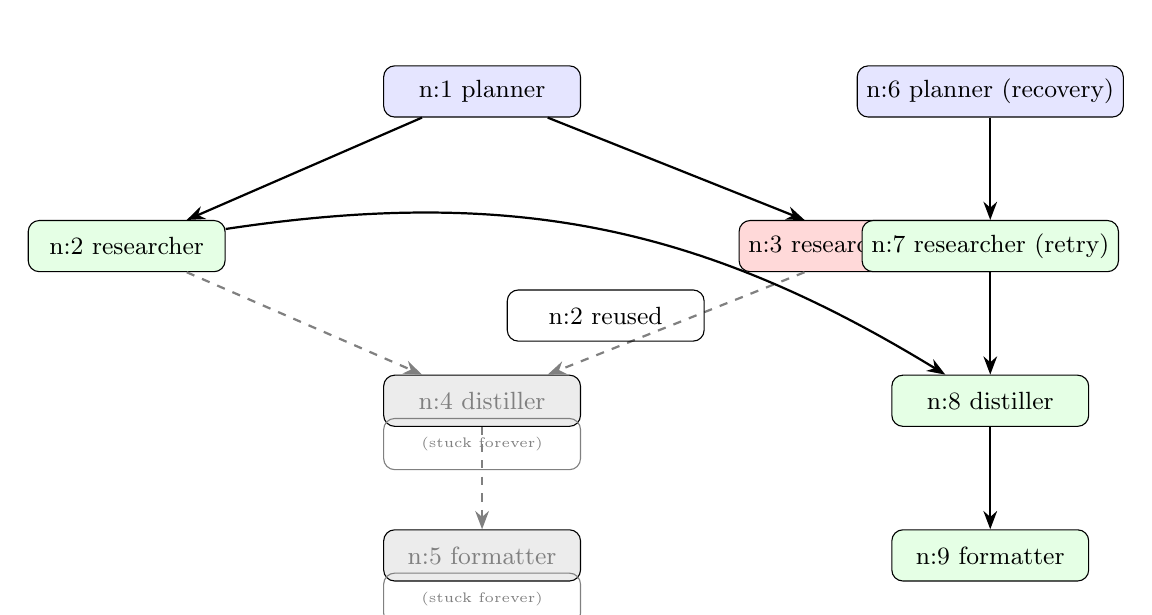
\begin{tikzpicture}[
  node distance=1.3cm and 2.0cm,
  every node/.style={draw, rounded corners, minimum width=2.5cm, minimum height=0.65cm,
    font=\small},
  arrow/.style={-Stealth, thick},
  stuck/.style={fill=gray!15, text=gray},
  active/.style={fill=green!10},
  failed/.style={fill=red!15},
  recovery/.style={fill=blue!10},
]
  \node (p1) [recovery] {n:1 planner};
  \node (r1) [active, below left=of p1]  {n:2 researcher};
  \node (r2) [failed, below right=of p1] {n:3 researcher (failed)};
  \node (d1) [stuck, below right=of r1]  {n:4 distiller};
  \node (f1) [stuck, below=of d1]        {n:5 formatter};

  \node (p2) [recovery, right=3.5cm of p1] {n:6 planner (recovery)};
  \node (r3) [active, below=of p2]  {n:7 researcher (retry)};
  \node (d2) [active, below=of r3]  {n:8 distiller};
  \node (f2) [active, below=of d2]  {n:9 formatter};

  \draw[arrow] (p1) -- (r1);
  \draw[arrow] (p1) -- (r2);
  \draw[arrow, gray, dashed] (r1) -- (d1);
  \draw[arrow, gray, dashed] (r2) -- (d1);
  \draw[arrow, gray, dashed] (d1) -- (f1);

  \draw[arrow] (p2) -- (r3);
  \draw[arrow] (r3) -- (d2);
  \draw[arrow] (d2) -- (f2);
  \draw[arrow, bend left=20] (r1) to (d2);  % n:2 reused in recovery branch

  \node[font=\tiny, gray] at ($(d1)+(0,-0.55)$) {(stuck forever)};
  \node[font=\tiny, gray] at ($(f1)+(0,-0.55)$) {(stuck forever)};
  \node[font=\tiny] at ($(r1)!0.5!(d2)+(0.6,0.1)$) {\small n:2 reused};
\end{tikzpicture}
\end{center}

% ─────────────────────────────────────────────────────────────────────────────
\section{Critic Failure Recovery}
% ─────────────────────────────────────────────────────────────────────────────

The critic failure path is distinct from node failure and is handled by
\mbox{\texttt{handle\_critic\_verdict()}} in \texttt{recovery.py}.

\begin{lstlisting}[style=pycode, caption={Critic-fail recovery — recovery.py:97--135}]
def handle_critic_verdict(nid, result, graph, recovered_branches, cap_hit):
    if result.output.get("verdict", "pass") != "fail":
        return False   # pass -> normal flow

    # Mark the child node (the one the critic was gating) as skipped
    graph.mark(child_nid, "skipped")

    # First failure on this target: queue a recovery Planner
    if target_nid and not recovered_branches.get(target_nid):
        recovered_branches[target_nid] = True
        rec_nid = graph.add_node("planner",
                                 inputs=["USER_QUERY"],
                                 metadata={"failure_report": fr,
                                           "recovers": target_nid,
                                           "recovery_reason": "critic_fail"})
    else:
        # Already recovered once and critic failed again -> cap hit, skip
        cap_hit.append(target_nid)
\end{lstlisting}

\begin{center}
\begin{tabular}{>{\bfseries}p{3.5cm} p{9.5cm}}
\toprule
Scenario & Behaviour \\
\midrule
Critic says \texttt{pass} & Child node becomes ready; normal flow continues \\
Critic says \texttt{fail} (first time) & Child marked \texttt{skipped}; recovery
  Planner queued with \texttt{inputs=[USER\_QUERY]} \\
Critic says \texttt{fail} (second time) & Cap hit; branch skipped entirely;
  final answer reflects missing data \\
\bottomrule
\end{tabular}
\end{center}

% ─────────────────────────────────────────────────────────────────────────────
\section{Input Resolution in Detail}
% ─────────────────────────────────────────────────────────────────────────────

\texttt{resolve\_inputs()} in \texttt{skills.py} materialises each input
reference into a dict for the prompt:

\begin{lstlisting}[style=pycode, caption={Input resolution — skills.py:77--110}]
def resolve_inputs(node_inputs, graph_nodes, query):
    for inp in node_inputs:
        if inp == "USER_QUERY":
            # literal: the original query text
            out.append({"id": "USER_QUERY", "kind": "query", "value": query})

        elif inp.startswith("n:") and inp in graph_nodes:
            # upstream node: pull its AgentResult.output
            upstream = graph_nodes[inp].get("result")
            out.append({"id": inp, "kind": "upstream",
                        "skill": upstream.agent_name, "output": upstream.output})

        elif inp.startswith("art:"):
            # artifact: bytes from content-addressable store, decoded as utf-8
            blob = artifacts_svc.get_bytes(inp)
            out.append({"id": inp, "kind": "artifact", "text": blob.decode(...)})

        else:
            # free-form literal: pass through unchanged
            out.append({"id": inp, "kind": "literal", "value": inp})
\end{lstlisting}

\begin{center}
\begin{tabular}{>{\ttfamily}p{3cm} p{9.5cm}}
\toprule
\normalfont\textbf{Input form} & \normalfont\textbf{What the skill receives} \\
\midrule
USER\_QUERY  & The original user query string \\
n:2          & The full \texttt{AgentResult.output} dict from node n:2 \\
art:sha256.. & The raw bytes of a stored artifact, decoded to text \\
anything else & Passed through as a literal string \\
\bottomrule
\end{tabular}
\end{center}

% ─────────────────────────────────────────────────────────────────────────────
\section{Session Persistence}
% ─────────────────────────────────────────────────────────────────────────────

Every run is associated with a session ID. The \texttt{SessionStore} in
\texttt{persistence.py} writes:

\begin{itemize}[noitemsep]
  \item \textbf{graph.pkl} — the full NetworkX DiGraph (for resume support)
  \item \textbf{query.txt} — the original user query
  \item \textbf{nodes/\{nid\}.json} — per-node result snapshots
\end{itemize}

A run can be resumed with \texttt{--resume <session\_id>}. The orchestrator
reloads the graph, resets any \texttt{running} nodes back to \texttt{pending}
(in case of a crash mid-run), and re-reads the original query.

% ─────────────────────────────────────────────────────────────────────────────
\section{Interview-Ready Summary}
% ─────────────────────────────────────────────────────────────────────────────

\begin{notebox}
\textbf{Questions you should be able to answer confidently:}
\end{notebox}

\begin{enumerate}
  \item \textbf{What is an orchestrator?} \\
    A component that manages what runs, when, and with what inputs — without
    doing the actual work. It sits above the workers (LLMs/skills) and below
    the user.

  \item \textbf{What does the Planner do and when?} \\
    The Planner runs first, receives only \texttt{USER\_QUERY}, and emits the
    \emph{entire DAG upfront} — all nodes and their dependency edges — in one
    LLM call. It is also re-invoked on node failure (recovery) or critic failure.

  \item \textbf{How does the execution loop work?} \\
    While there are ready nodes (predecessors all complete/skipped), fire all
    ready nodes in parallel via \texttt{asyncio.gather}. Collect results, update
    statuses, extend the graph. Repeat until nothing is ready and nothing is
    running.

  \item \textbf{How is context kept small per LLM?} \\
    Each node's inputs list is explicit and minimal. \texttt{resolve\_inputs}
    only materialises what is listed — not the full graph. A 10-node graph does
    not mean any LLM sees 10 nodes' worth of tokens.

  \item \textbf{How does recovery work?} \\
    On upstream failure, the orchestrator collects prior completed node IDs and
    adds a new Planner node with \texttt{inputs = [USER\_QUERY] + prior\_complete}
    and a short failure report. The recovery Planner receives the failure context
    and the already-computed data, then emits a targeted recovery DAG. The old
    stuck nodes are left behind.

  \item \textbf{What is critic auto-insertion?} \\
    When a skill with \texttt{critic: true} (e.g.\ distiller) completes, the
    orchestrator automatically inserts a Critic node on every outgoing edge,
    without any skill requesting it. The Critic evaluates quality; on fail it
    marks the child skipped and queues a recovery Planner.

  \item \textbf{What happens to stuck nodes after failure?} \\
    If a node's predecessor is \texttt{failed} (not \texttt{skipped}), the node
    is never added to \mbox{\texttt{ready\_nodes}} and simply stays \texttt{pending}
    forever. The loop exits naturally when no nodes are ready and none are
    running.
\end{enumerate}

% ─────────────────────────────────────────────────────────────────────────────
\section{Quick Reference: Key Files}
% ─────────────────────────────────────────────────────────────────────────────

\begin{center}
\begin{tabular}{>{\ttfamily}p{5cm} p{8.5cm}}
\toprule
\normalfont\textbf{File} & \normalfont\textbf{Responsibility} \\
\midrule
flow.py         & Orchestrator (\texttt{Graph} + \texttt{Executor}). The main loop,
                  node scheduling, critic insertion, recovery dispatch. \\
skills.py       & Skill registry, input resolution, prompt rendering, LLM dispatch. \\
recovery.py     & Failure classification and recovery decision logic. \\
schemas.py      & \texttt{AgentResult}, \texttt{NodeSpec}, \texttt{NodeState} data models. \\
persistence.py  & Session storage (graph.pkl, node snapshots). \\
memory.py       & FAISS-backed memory read/write. \\
agent\_config.yaml & Skill definitions, tools, critic flags, internal successors. \\
\midrule
llm\_gatewayV9/main.py    & FastAPI gateway. Provider failover, routing, rate limiting. \\
llm\_gatewayV9/router.py  & Router logic: tier classification, provider selection. \\
llm\_gatewayV9/providers.py & Per-provider adapter implementations. \\
\bottomrule
\end{tabular}
\end{center}

\end{document}
